\documentclass{beamer}

\usetheme{AnnArbor}
\usecolortheme{whale}
%% https://deic.uab.cat/~iblanes/beamer_gallery/index_by_theme_and_color.html

\author{Sean Laverty}
\title{Day \#9: more beamer}
\date{Wednesday, September 20, 2023}

\begin{document}

\frame{\maketitle}

\frame{\frametitle{Acknowledgements}
Experiment with theme and color, and itemize enumerate to observe changes.

\begin{itemize} %% <"click"> vs <"click"-> dash means "and stays"
\item<1-> Funding sources
\item<2-> People that helped
\item<3-> Institutions or organizations
\end{itemize}
}

\section{Introduction}

\frame{\frametitle{Literature review}
This slide might contain a brief list of facts we summarize from literature.
\begin{itemize}
\item I just wrote a sentence.  I want to be careful writing long sentences.
\item Instead of a bibliography, we might use footnotes\footnote{This is a footnote. This also works in article.}.
\end{itemize}
}

\section{Big Question (Hypothesis)}
\frame{\frametitle{What is it?}
All of our text formatting commands still work.
\vfill

We can use \textcolor{blue}{colored text}.
\vfill

We can use special fonts like \textit{italics}.
\vfill

Presentations come with one new trick, called \alert<2>{alert}.
\vfill

}

\section{Methods or Approach}

\frame{\frametitle{Formatting with minipage}

\begin{minipage}{0.28\textwidth}

\begin{itemize}
\item               hey
\item look
\item an image
\end{itemize}

\end{minipage}\hfill\vrule\hfill %% gives a vertical separator
%% no white space between minipages
\begin{minipage}{0.68\textwidth}
%\centering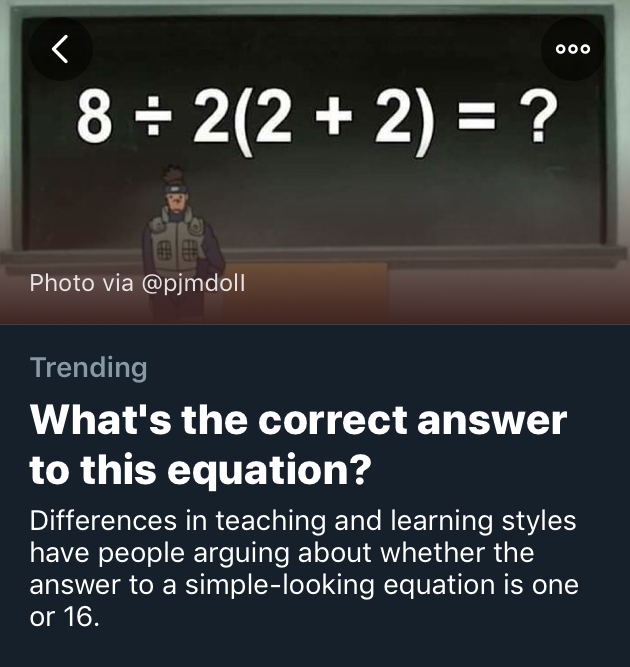
\includegraphics[width = 0.6\textwidth]{twitter.png}
\centering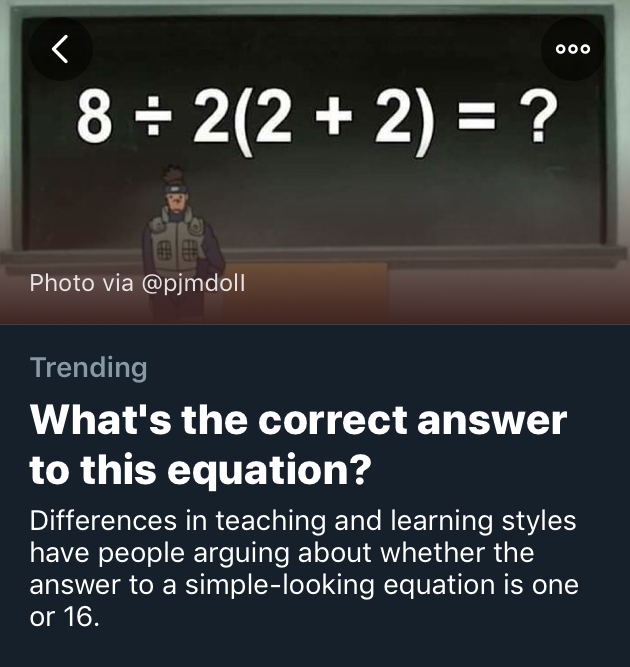
\includegraphics[height = 0.6\textheight]{twitter.png}
%% a nicer way to introduce images that preserves layout
%%\uncover<2>{\centering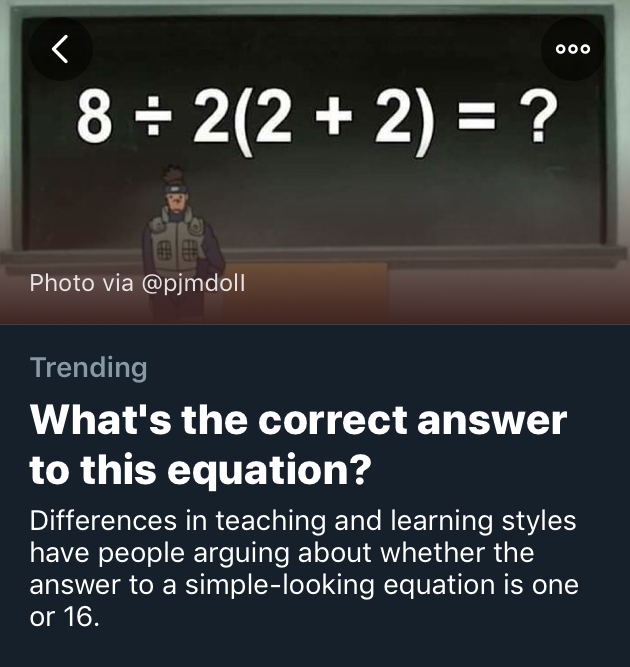
\includegraphics[height = 0.6\textheight]{twitter.png}}
\end{minipage}
\vfill

Note: We aren't going to use the figure environment, a formal caption, or a label (most likely).
}

\section{Results}
\frame{\frametitle{Don't forget about math}
We can include math as well,
\[x = \frac{-b \pm \sqrt{b^2 - 4ac}}{2a},\]

which solves \(ax^2 + bx + c = 0 \) for \(x\).
}


\section{Conclusions}

\frame{\frametitle{Warnings}
\begin{itemize}
\item Too much text is often hard to read.
\item Tables aren't often as useful in slides as on paper.  \alert<2>{If you do, avoid too many vertical separator bars.}
\item If references are relevant, list them.
\item Lots of people include QR codes (or short-links).
\end{itemize}
}

%% added after class, prompted by questions
\frame{\frametitle{Extra stuff}
\onslide<1->{All of our text formatting commands still work.}
\vfill

\onslide<4>{We can use \textcolor{blue}{colored text}.}
\vfill

\onslide<2->{We can use special fonts like \textit{italics}.}
\vfill

\onslide<3->{Presentations come with one new trick, called \alert<2>{alert}.}
\vfill

%% Allows for alternate content on clicks
\alt<2>{Cat}{Dog}
%% \alt<2>{\textcolor{red}{Note}}{\textcolor{blue}{Note}}
}

\end{document}